\documentclass{slide}
\usepackage{tikz}

\title{Course Overview}
\subtitle{Software Architecture}
\institute{University of Queensland}
\author{Richard Thomas}
\date{\week{1}}
\titlegraphic {
    \begin{tikzpicture}[overlay,remember picture]
    \node[left=0.1cm] at (current page.-9){
        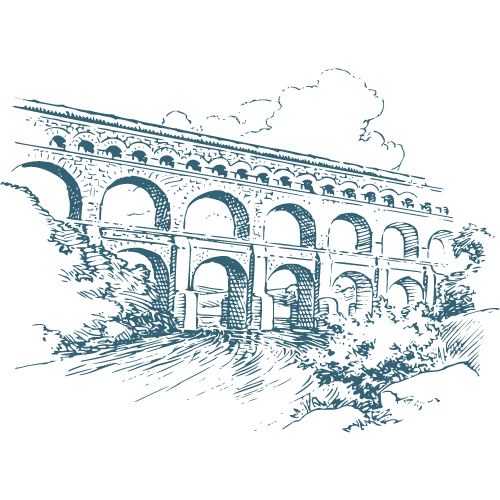
\includegraphics[width=4.75cm]{images/course-logo.png}
    };
    \end{tikzpicture}
}

\begin{document}

\maketitle

\begin{frame}{What is the course about?}
\Large
\begin{itemize}[<+->]
    \item Well, \highlight{software architecture}.
	\vspace{2mm}
    \item Designing and building software systems.
    \begin{itemize}
        \large \item Multiple \highlight{software components} that work together.
    \end{itemize}
    \item Using \highlight{architecture patterns} to structure software systems to be \highlight{maintainable}.
    \item How to build software that is \highlight{reliable} and \highlight{fault tolerant}.
    \item How to build software that is \highlight{scalable}.
\end{itemize}
\end{frame}

\begin{frame}{What will we be doing?}

{\color{pine} Lectures}
\begin{itemize}[<+->]
    \item Learn common \highlight{architecture patterns}.
    \item Learn tools and techniques for \highlight{designing} and \highlight{implementing} software systems.
    \item Learn the principles for working with \highlight{distributed systems}.
\end{itemize}

{\color{pine} Case Studies}
\begin{itemize}[<+->]
    \item Work on \highlight{case studies} that implement architectual patterns.
    \item Hands-on practice with the tools and techniques for \highlight{designing} and \highlight{implementing} software systems.
\end{itemize}

{\color{pine} Practicals}
\begin{itemize}[<+->]
    \item Develop stateless and persistent \highlight{RESTful web APIs}.
    \item Package software components into \highlight{Docker} containers.
    \item Deploy containers to cloud platforms using \highlight{Terraform}.
    \item Use cloud platform tools to \highlight{monitor} and \highlight{scale} applications.
\end{itemize}

\end{frame}

\section{Assessment}

\begin{frame}{Assessment}
\begin{tabular}{lr}
\Large{Project Proposal} & \hspace{2em}\Large{5\%} \\
 & \\
\Large{Cloud Infrastructure Assignment} & \Large{35\%} \\
\hspace{1em} API Functionality & 14\% \\
\hspace{1em} Deployed to Cloud & 8.75\% \\
\hspace{1em} Scalable Application & 12.25\% \\
 & \\
\Large{Architecture Presentation} & \Large{25\%} \\
 & \\
\Large{Capstone Project} & \Large{35\%} \\
(Delivering Quality Attributes Project) &  \\
\end{tabular}
\end{frame}

\point[\huge{Building a Scalable Architecture}]{
    \vspace{1em}
    \Large
    \begin{enumerate}
        \item Build a \highlight{RESTful web API} according to our specification.
        \item \highlight{Test} that the API satisfies the specification.
        \item \highlight{Deploy} the API to a cloud platform.
        \item \highlight{Scale} the API to handle \highlight{high loads}.
    \end{enumerate}
}

\point[\huge{Capstone Project}]{
    \vspace{1em}
    \Large
    \begin{enumerate}
        \item \highlight{Propose} a \highlight{software system} that you would like to build.
        \item Vote on other proposals on which you would like to work.
        \item Teams will be assigned to work on selected projects.
        \item \highlight{Design} and \highlight{implement} the project.
    \end{enumerate}
}

\point[\huge{Architecture Presentation}]{
    \vspace{1em}
    \Large
    \begin{itemize}
        \item Team presents details of project architecture.
    			\begin{itemize}
       			\large{\item \highlight{Everyone} presents.}
    			\end{itemize}
        \vspace{2mm}
        \item \highlight{Individuals} present on different sets of questions.
    			\begin{itemize}
       			\large{\item Compare and contrast with another architectural pattern.}
                \vspace{1mm}
       			\large{\item Pros and cons of architecture.}
                \vspace{1mm}
       			\large{\item Implementation characteristics of design.}
                \vspace{1mm}
       			\large{\item Potential security risks of architecture.}
    			\end{itemize}
        \vspace{2mm}
        \item \highlight{Everyone} is expected to understand entire architecture.
    			\begin{itemize}
       			\large{\item Questions can be directed to \highlight{anyone}.}
    			\end{itemize}
    \end{itemize}
% Pre-2025 Presentation Details
%    \begin{enumerate}
%        \item Find an active \highlight{open-source} project that \highlight{interests you}.
%    			\begin{itemize}
%       			\large{\item From a list of suggested projects.}
%    			\end{itemize}
%       \item \highlight{Discuss} the project with course staff.
%        \item Dive into the code and \highlight{understand} the architecture.
%        \item \highlight{Present} a summary of the architecture to the class.
%    \end{enumerate}
}

\section{You and Us}

\point[Who are we?]{
    \vspace{-1cm}
    \Large
    \centering
    \begin{minipage}{0.35\textwidth}
    \begin{center}
    \begin{tikzpicture}
    \clip (0,0) circle (1.5cm) node {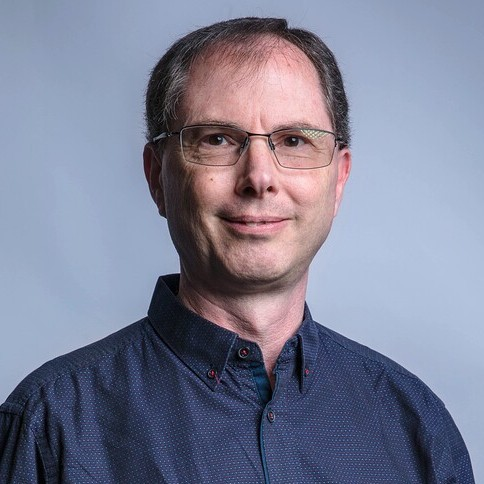
\includegraphics[width=3cm]{images/richard.jpeg}};
    \end{tikzpicture}

    Richard Thomas
    \end{center}
    \end{minipage}
%
    \begin{minipage}{0.35\textwidth}
    \begin{center}
    \begin{tikzpicture}
    \clip (0,0) circle (1.5cm) node {
\includegraphics[width=3cm]{images/evan.jpeg}};
    \end{tikzpicture}

    Evan Hughes
    \end{center}
    \end{minipage}
%

    \begin{minipage}{0.35\textwidth}
    \begin{center}
    \begin{tikzpicture}
    \clip (0,0) circle (1.5cm) node {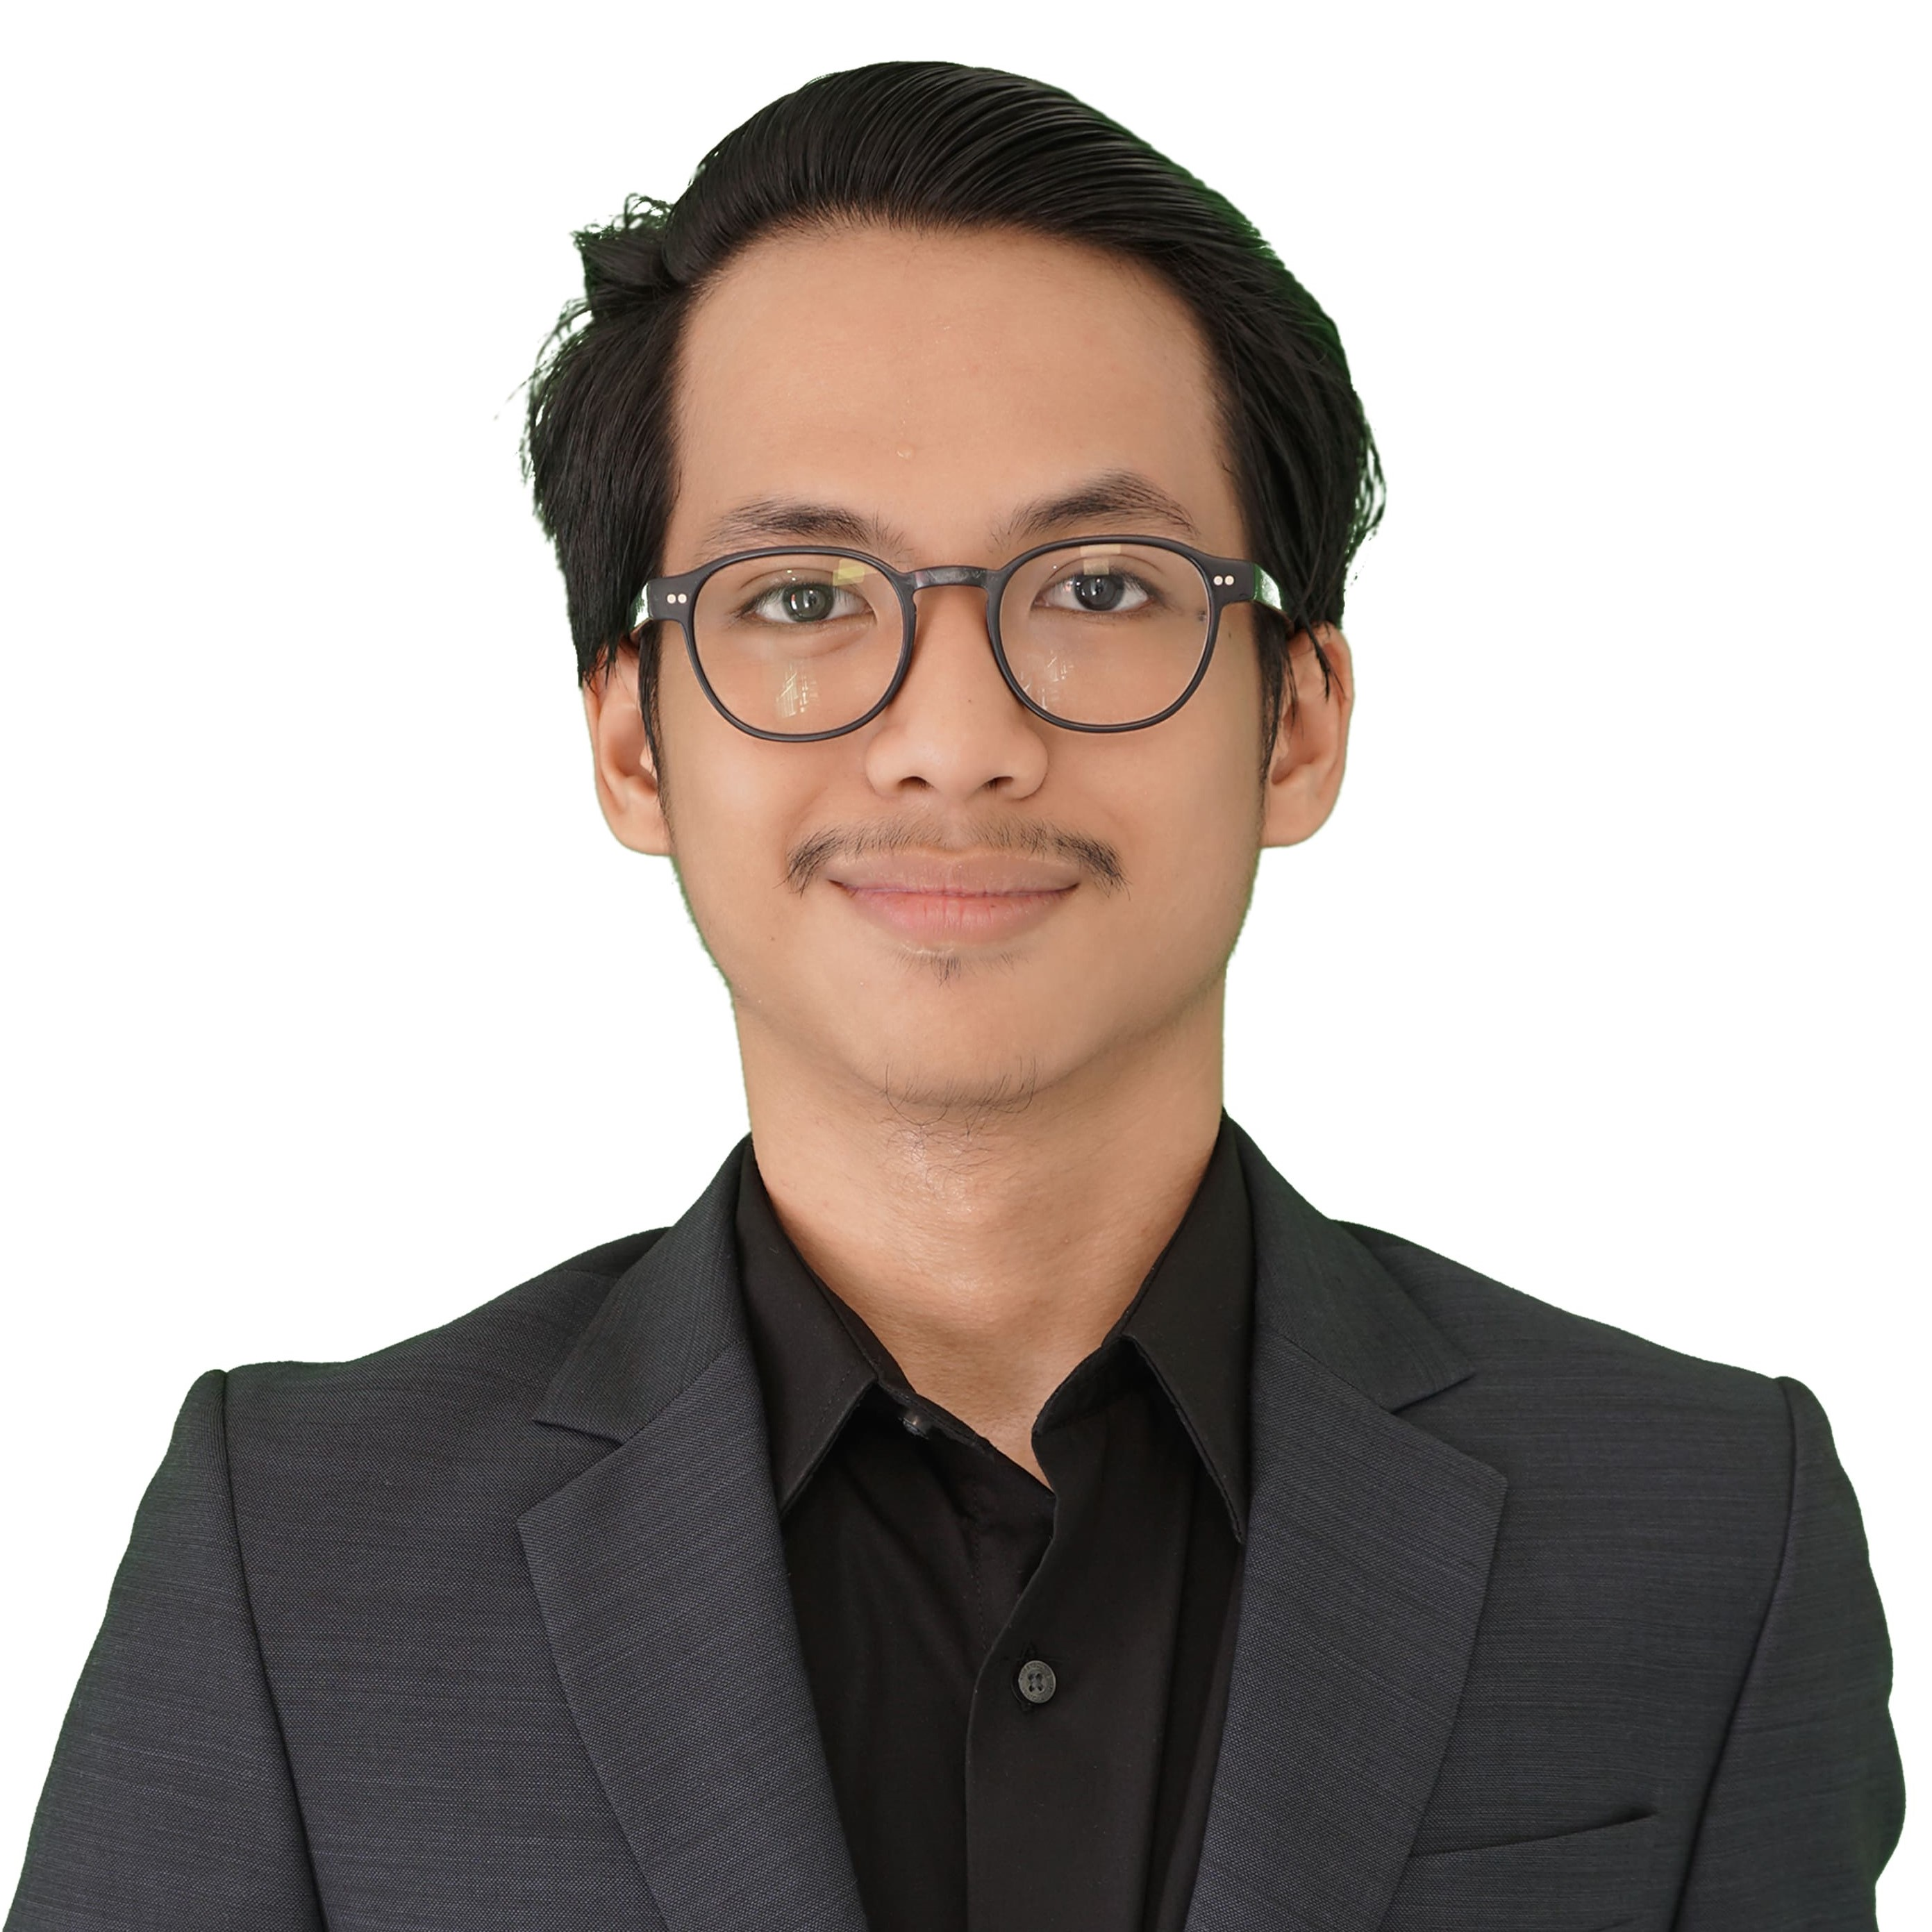
\includegraphics[width=3cm]{images/riza.jpeg}};
    \end{tikzpicture}

    Riza Wibawa
    \end{center}
    \end{minipage}
%
    \begin{minipage}{0.35\textwidth}
    \begin{center}
    \begin{tikzpicture}
    \clip (0,0) circle (1.5cm) node {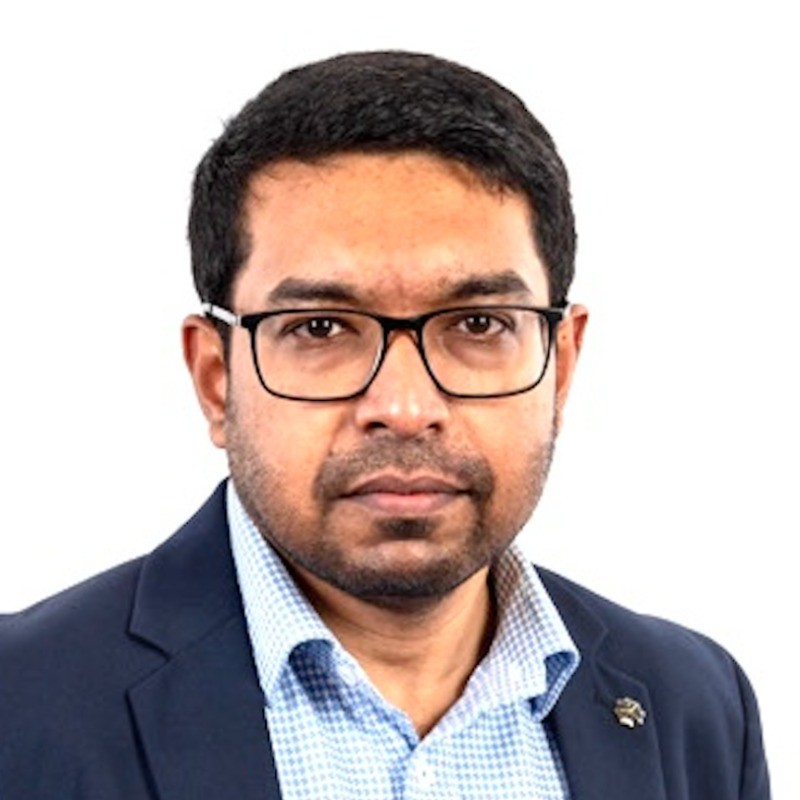
\includegraphics[width=3cm]{images/zaidul.jpeg}};
    \end{tikzpicture}

    Zaidul Alam
    \end{center}
    \end{minipage}
}

\question{Who are \highlight{you}?}

%\image[height=\textheight]{images/courses_with_duals.png}

%\image[height=\textheight]{images/majors.png}

%\image{images/previous_courses.png}

%\image{images/year_of_study.png}

%\image{images/important_courses.png}

\point[\huge{Course Website}]{
    \vspace{1em}
    \Large
    All course material is hosted on the course website:
    {\color{pine}\url{https://csse6400.uqcloud.net}}

    \hfill

    If you find any \highlight{errors} or have any \highlight{improvements},
    please submit a pull request on GitHub:
    {\color{pine}\url{https://github.com/CSSE6400/software-architecture}}
}

\begin{frame}{GitHub Username Registration Form}
\Large
You need access to the CSSE6400 organisation on GitHub.
\begin{itemize}
    \item \highlight{Practicals} -- Access to code.
    \item \highlight{Assessment} -- Most submissions.
\end{itemize}
\vspace{5mm}
\centering

\includegraphics[trim=50 50 50 50,clip,height=0.4\textheight]{images/reg_form_qr.png}

{\color{pine}\url{https://tiny.cc/csse6400reg}}
\end{frame}


%\references{articles,books}

\end{document}
